\chapter{Schiere di antenne}

	Vedremo in questo capitolo come combinare in modo opportuno una serie di antenne per migliorare le prestazioni del nostro ricevitore.

\section{Schiera di antenne isotrope}
	Il primo caso che analizzeremo è quello di una serie lineare ed equispaziata di antenne isotrope, ovvero antenne che irradiano in modo uniforme in tutte le direzioni.

	Questa semplificazione permette di considerare le proprietà del posizionamento delle antenne nell'\emph{array} astraendo dalle caratteristiche specifiche delle varie antenne.

	\begin{figure}[ht]
		\centering
		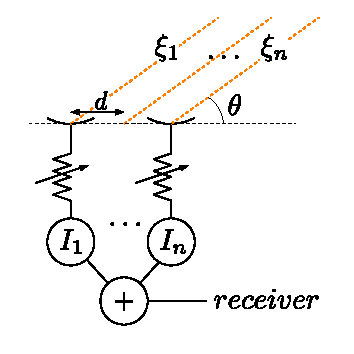
\includegraphics{img/schiera_antenne.pdf}
		\caption{Le antenne della schiera sono alimentate dalle correnti $I_i$ e ricevono il segnale dal campo lontano con sfasamenti diversi $\xi_i$.}
		\label{fig:schiera}
	\end{figure}

	Dallo schema elettrico in figura \ref{fig:schiera} si può facilmente calcolare il segnale in arrivo al ricevitore, definito come \gls{af}.

	\begin{esp} \label{eq:array_factor}
		AF = \sum_{i=1}^n I_i e^{\jmath \xi_i}
			\stackrel{(*)}{=} \sum_{i=1}^n I_i ~ e^{\jmath (i-1) \beta d \cos \theta}
	\end{esp}
	dove in (*) si calcola la differenza di cammino tra i vari percorsi.

	D'ora in avanti considereremo sempre alimentazioni $I_i$ sfasate tra loro di un angolo $\alpha$ costante: in questo caso il calcolo dell'\gls{af} si riduce a

	\begin{esp}
		AF = \sum_{i=0}^{n-1} A_i ~ e^{\jmath i (\beta d \cos \theta + \alpha)}
			\stackrel{.}{=} \sum_{i=0}^{n-1} ~ e^{\jmath i \psi}
	\end{esp}
	dove $I_i$ viene scomposto in modulo e fase come $A_i ~ e^{\jmath (i-1) \alpha}$ e $\psi$ è un angolo definito per semplificare la notazione che racchiude le tutti gli sfasamenti.
	
	\subsection{Regione di visibilità}
		I valori validi per l'inclinazione rispetto all'array sono $\theta \in [0, \pi]$, perché i valori opposti sono ottenuti semplicemente per simmetria.s
		
		Questo induce dei limiti nell'angolo $\psi$: il range di valori validi per questo angolo è detto \emph{regione di visibilità}.
		\begin{equation} \begin{gathered}
		 0 \le \theta \le \pi \\
		 -\beta d \le \beta d \cos \theta \le \beta d \\ 
		 \alpha - \beta d \le \psi \le \alpha + \beta d 
		\end{gathered} \end{equation}

	\subsection{Modulo uniforme delle correnti}
		Nel caso particolare in cui le correnti abbiano modulo uguale e sfasamento $\alpha$, il calcolo dell'\gls{af} si semplifica ulteriormente.
			
		\begin{esp}
			AF 
				= A_o \sum_{i=0}^{n-1} ~ e^{\jmath i \psi}
				= A_o \frac{1 - ~ e^{\jmath n \psi}}{1 - ~ e^{\jmath \psi}}
				= A_o 
					\frac{e^{\jmath n/2 \psi}}{e^{\jmath \psi}} 
					\frac{e^{\jmath n/2 \psi} - e^{- \jmath n/2 \psi}}{e^{\jmath \psi} - e^{-\jmath \psi}} 
				= A_o 
					\frac{e^{\jmath n/2 \psi}}{e^{\jmath \psi}} 
					\frac{\sen(n/2 \psi)}{\sen(\psi/2)} \frac{e^{\jmath n/2 \psi}}{e^{\jmath \psi}} 
				= 
				
		\end{esp}